\documentclass[journal,12pt,twocolumn]{IEEEtran}

\usepackage{setspace}
\usepackage{gensymb}
\singlespacing
\usepackage[cmex10]{amsmath}

\usepackage{amsthm}

\usepackage{mathrsfs}
\usepackage{txfonts}
\usepackage{amsmath}
\usepackage{stfloats}
\usepackage{float} 
\usepackage{bm}
\usepackage{tikz}
\usepackage{pgfplots}
\usepackage{cite}
\usepackage{cases}
\usepackage{subfig}

\usepackage{longtable}
\usepackage{multirow}

\usepackage{enumitem}
\usepackage{mathtools}
\usepackage{steinmetz}
\usepackage{tikz}
\usepackage{circuitikz}
\usepackage{verbatim}
\usepackage{tfrupee}
\usepackage[breaklinks=true]{hyperref}
\usepackage{graphicx}
\usepackage{tkz-euclide}

\usetikzlibrary{calc,math}
\usepackage{listings}
    \usepackage{color}                                            %%
    \usepackage{array}                                            %%
    \usepackage{longtable}                                        %%
    \usepackage{calc}                                             %%
    \usepackage{multirow}                                         %%
    \usepackage{hhline}                                           %%
    \usepackage{ifthen}                                           %%
    \usepackage{lscape}     
\usepackage{multicol}
\usepackage{chngcntr}
\usepackage{hyperref}
\hypersetup{
    colorlinks=true,
    linkcolor=blue,
    filecolor=blue,      
    urlcolor=blue,
}
\DeclareMathOperator*{\Res}{Res}

\renewcommand\thesection{\arabic{section}}
\renewcommand\thesubsection{\thesection.\arabic{subsection}}
\renewcommand\thesubsubsection{\thesubsection.\arabic{subsubsection}}

\renewcommand\thesectiondis{\arabic{section}}
\renewcommand\thesubsectiondis{\thesectiondis.\arabic{subsection}}
\renewcommand\thesubsubsectiondis{\thesubsectiondis.\arabic{subsubsection}}


\hyphenation{op-tical net-works semi-conduc-tor}
\def\inputGnumericTable{}                                 %%

\lstset{
%language=C,
frame=single, 
breaklines=true,
columns=fullflexible
}

\makeatletter
\setlength{\@fptop}{0pt}
\makeatother

\begin{document}


\newtheorem{theorem}{Theorem}[section]
\newtheorem{problem}{Problem}
\newtheorem{proposition}{Proposition}[section]
\newtheorem{lemma}{Lemma}[section]
\newtheorem{corollary}[theorem]{Corollary}
\newtheorem{example}{Example}[section]
\newtheorem{definition}[problem]{Definition}

\newcommand{\BEQA}{\begin{eqnarray}}
\newcommand{\EEQA}{\end{eqnarray}}
\newcommand{\define}{\stackrel{\triangle}{=}}
\bibliographystyle{IEEEtran}
\raggedbottom
\setlength{\parindent}{0pt}
\providecommand{\mbf}{\mathbf}
\providecommand{\pr}[1]{\ensuremath{\Pr\left(#1\right)}}
\providecommand{\qfunc}[1]{\ensuremath{Q\left(#1\right)}}
\providecommand{\sbrak}[1]{\ensuremath{{}\left[#1\right]}}
\providecommand{\lsbrak}[1]{\ensuremath{{}\left[#1\right.}}
\providecommand{\rsbrak}[1]{\ensuremath{{}\left.#1\right]}}
\providecommand{\brak}[1]{\ensuremath{\left(#1\right)}}
\providecommand{\lbrak}[1]{\ensuremath{\left(#1\right.}}
\providecommand{\rbrak}[1]{\ensuremath{\left.#1\right)}}
\providecommand{\cbrak}[1]{\ensuremath{\left\{#1\right\}}}
\providecommand{\lcbrak}[1]{\ensuremath{\left\{#1\right.}}
\providecommand{\rcbrak}[1]{\ensuremath{\left.#1\right\}}}
\theoremstyle{remark}
\newtheorem{rem}{Remark}
\newcommand{\sgn}{\mathop{\mathrm{sgn}}}
\providecommand{\abs}[1]{$\left\vert#1\right\vert$}
\providecommand{\res}[1]{\Res\displaylimits_{#1}} 
%\providecommand{\norm}[1]{$\left\lVert#1\right\rVert$}
\providecommand{\norm}[1]{\lVert#1\rVert}
\providecommand{\mtx}[1]{\mathbf{#1}}
\providecommand{\mean}[1]{$E\left[ #1 \right]$}
\providecommand{\fourier}{\overset{\mathcal{F}}{ \rightleftharpoons}}
%\providecommand{\hilbert}{\overset{\mathcal{H}}{ \rightleftharpoons}}
\providecommand{\system}{\overset{\mathcal{H}}{ \longleftrightarrow}}
	%\newcommand{\solution}[2]{\textbf{Solution:}{#1}}
\newcommand{\solution}{\noindent \textbf{Solution: }}
\newcommand{\cosec}{\,\text{cosec}\,}
\providecommand{\dec}[2]{\ensuremath{\overset{#1}{\underset{#2}{\gtrless}}}}
\newcommand{\myvec}[1]{\ensuremath{\begin{pmatrix}#1\end{pmatrix}}}
\newcommand{\mydet}[1]{\ensuremath{\begin{vmatrix}#1\end{vmatrix}}}
\newcommand*{\permcomb}[4][0mu]{{{}^{#3}\mkern#1#2_{#4}}}
\newcommand*{\perm}[1][-3mu]{\permcomb[#1]{P}}
\newcommand*{\comb}[1][-1mu]{\permcomb[#1]{C}}
\numberwithin{equation}{subsection}
\makeatletter
\@addtoreset{figure}{problem}
\makeatother
\let\StandardTheFigure\thefigure
\let\vec\mathbf
\renewcommand{\thefigure}{\theproblem}
\def\putbox#1#2#3{\makebox[0in][l]{\makebox[#1][l]{}\raisebox{\baselineskip}[0in][0in]{\raisebox{#2}[0in][0in]{#3}}}}
     \def\rightbox#1{\makebox[0in][r]{#1}}
     \def\centbox#1{\makebox[0in]{#1}}
     \def\topbox#1{\raisebox{-\baselineskip}[0in][0in]{#1}}
     \def\midbox#1{\raisebox{-0.5\baselineskip}[0in][0in]{#1}}
\vspace{3cm}
\title{Assignment 3}
\author{Sachin Karumanchi - AI20BTECH11013}
\maketitle
\newpage
\bigskip
\renewcommand{\thefigure}{\theenumi}
\renewcommand{\thetable}{\theenumi}
Download all python codes from
\begin{lstlisting}
https://github.com/sachinkarumanchi/EE3900/blob/main/assignment2.pdf
\end{lstlisting}
and latex codes from
\begin{lstlisting}
https://github.com/sachinkarumanchi/EE3900/blob/main/assignment2.tex
\end{lstlisting}
\section*{Problem(Matrices-2.22(2)}
Draw a line segment AB of length 8units. Taking $\Vec{A}$ as center, draw a circle of radius 4 units, taking $\Vec{B}$ as center draw another circle of radius 3 units. Construct tangents to each circle from the center of another circle. 
\section*{Solution}
Given, AB of lenght 8 units 
\begin{center}
\begin{tabular}{|c|c|c|c|}
  \hline
  & Symbol & Circle1 & Circle2 \\
  \hline
  Center & $\Vec{A},\Vec{B}$ & $\myvec{0\\0}$ & $\myvec{8\\0}$ \\ 
  \hline
  Radius & r1,r2 & 4 & 3 \\ 
  \hline
\end{tabular}
\end{center}
Let BP,BQ be the tangents at to the circle with center $\Vec{A}$\\
Now,$\Vec{AP}$ and $\vec{PB}$ are perpendicular so
\begin{align}
    (\vec{A}-\vec{P})^T (\vec{P}-\vec{B}) &= 0
\end{align}
Since $\norm{\vec{P}^2}=16$
\begin{align}
    \implies \vec{B}^T \vec{P} &= 16\\
    \implies \myvec{1&0} \vec{P} &= 2
\end{align}
Now re-write $\vec{P}$ as
\begin{align}
    \implies \Vec{P} &=\vec{q_1}+\lambda_1\vec{m_1}
\end{align}
\begin{align}
    \implies \vec{P} &= \myvec{2\\0} + \lambda_1 \myvec{0\\1} \label{eq1}
\end{align}
where $\vec{q_1}=\myvec{2\\ 0},\vec{m_1}=\myvec{0\\1}$
We know,
\begin{align}
    \norm{\vec{q_1}+\lambda\vec{m_1}}^2&=r_1^2\\
    (\vec{q_1}+\lambda_1\vec{m_1})^T(\vec{q_1}+\lambda_1 \vec{m_1})&=r_1^2\\
    \lambda_1^2&=\frac{r_1^2-\norm{\vec{q_1}}^2}{\norm{\vec{m_1}}^2}\\
    \lambda_1 &= \pm 3.46410
\end{align}
from \eqref{eq1}, The Points $\vec{P}$ and $\vec{Q}$ are
\begin{align}
    \vec{P}&=\myvec{2\\3.46410}\\
    \vec{Q}&=\myvec{2\\-3.46410}
\end{align}
Let AR,AS be the tangents to the circle with center $\vec{B}$\\
Shift the origin from $\vec{A}$ to $\vec{B}$\\
The new co-ordinates of $\vec{A}$ and $\vec{B}$ would be
\begin{align}
    \vec{A}&=\myvec{-8\\0}\\
    \vec{B}&=\myvec{0\\0}
\end{align}
Now similarly, as above $\vec{BR}$ is perpendicular to $\vec{RA}$
\begin{align}
    (\vec{B}-\vec{R})^T (\vec{R}-\vec{A}) &= 0
\end{align}
Since $\norm{\vec{R}^2}=9$
\begin{align}
    \implies \vec{A}^T \vec{R} &= 16\\
    \implies \myvec{1&0} \vec{R} &= -1.125
\end{align}
Now re-write $\vec{P}$ as
\begin{align}
    \implies \Vec{R} &=\vec{q_2}+\lambda_2\vec{m_2}
\end{align}
\begin{align}
    \implies \vec{R} &= \myvec{-1.125\\0} + \lambda_2 \myvec{0\\1} \label{eq2}
\end{align}
where $\vec{q_2}=\myvec{-1.125\\ 0},\vec{m_2}=\myvec{0\\1}$
We know,
\begin{align}
    \norm{\vec{q_2}+\lambda\vec{m_2}}^2&=r_2^2\\
    (\vec{q_2}+\lambda_2 \vec{m_2})^T(\vec{q_2}+\lambda_2 \vec{m_2})&=r_2^2\\
    \lambda_2^2&=\frac{r_2^2-\norm{\vec{q_2}}^2}{\norm{\vec{m_2}}^2}\\
    \lambda_2 &= \pm 2.78017
\end{align}
from \eqref{eq2}, The Points $\vec{R}$ and $\vec{S}$ are
\begin{align}
    \vec{R}&=\myvec{-1.125\\2.78107}\\
    \vec{S}&=\myvec{-1.125\\-2.78107}
\end{align}
Now shifting the origin to $\vec{A}$, The co-ordinates of $\vec{A,B,P,Q,R,S}$ would be
\begin{align}
    \vec{A}&=\myvec{0\\0}\\
    \vec{B}&=\myvec{8\\0}\\
    \vec{P}&=\myvec{2\\3.46140}\\
    \vec{Q}&=\myvec{2\\-3.46140}\\
    \vec{R}&=\myvec{6.875\\2.78107}\\
    \vec{S}&=\myvec{6.875\\-2.78107}
\end{align}
\begin{figure}
    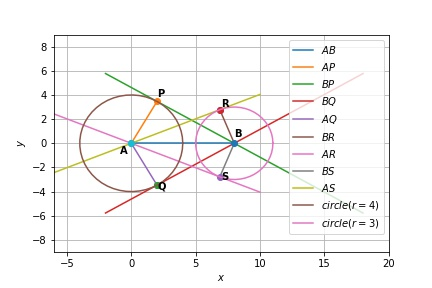
\includegraphics[width=11cm]{Assignment3.jpg}
    \label{plot1}
\end{figure}
\end{document}
